% This file was converted to LaTeX by Writer2LaTeX ver. 1.0.2
% see http://writer2latex.sourceforge.net for more info
\documentclass[twoside,letterpaper]{article}
\usepackage[latin1]{inputenc}
\usepackage[T1]{fontenc}
\usepackage[english]{babel}
\usepackage{amsmath}
\usepackage{amssymb,amsfonts,textcomp}
\usepackage{color}
\usepackage{array}
\usepackage{supertabular}
\usepackage{hhline}
\usepackage{hyperref}
\hypersetup{pdftex, colorlinks=true, linkcolor=blue, citecolor=blue, filecolor=blue, urlcolor=blue, pdftitle=SYSTEM AND SOFTWARE ARCHITECTURAL AND DETAILED DESIGN DESCRIPTION, pdfauthor=James Combs, pdfsubject=, pdfkeywords=}
\usepackage[pdftex]{graphicx}
% Outline numbering
\setcounter{secnumdepth}{5}
\renewcommand\thesection{\arabic{section}}
\renewcommand\thesubsection{\arabic{section}.\arabic{subsection}}
\renewcommand\thesubsubsection{\arabic{section}.\arabic{subsection}.\arabic{subsubsection}}
\renewcommand\theparagraph{\arabic{section}.\arabic{subsection}.\arabic{subsubsection}.\arabic{paragraph}}
\renewcommand\thesubparagraph{\arabic{section}.\arabic{subsection}.\arabic{subsubsection}.\arabic{paragraph}.\arabic{subparagraph}}
\makeatletter
\newcommand\arraybslash{\let\\\@arraycr}
\makeatother
% List styles
\newcommand\liststyleWWviiiNumii{%
\renewcommand\theenumi{\arabic{enumi}}
\renewcommand\theenumii{\arabic{enumii}}
\renewcommand\theenumiii{\arabic{enumiii}}
\renewcommand\theenumiv{\arabic{enumiv}}
\renewcommand\labelenumi{\theenumi)}
\renewcommand\labelenumii{\theenumii.}
\renewcommand\labelenumiii{\theenumiii.}
\renewcommand\labelenumiv{\theenumiv.}
}
% Page layout (geometry)
\setlength\voffset{-1in}
\setlength\hoffset{-1in}
\setlength\topmargin{0.5in}
\setlength\oddsidemargin{1in}
\setlength\evensidemargin{1in}
\setlength\textheight{8.278in}
\setlength\textwidth{6.5in}
\setlength\footskip{0.561in}
\setlength\headheight{0.5in}
\setlength\headsep{0.461in}
% Footnote rule
\setlength{\skip\footins}{0.0469in}
\renewcommand\footnoterule{\vspace*{-0.0071in}\setlength\leftskip{0pt}\setlength\rightskip{0pt plus 1fil}\noindent\textcolor{black}{\rule{0.25\columnwidth}{0.0071in}}\vspace*{0.0398in}}
% Pages styles
\makeatletter
\newcommand\ps@Standard{
  \renewcommand\@oddhead{}
  \renewcommand\@evenhead{\@oddhead}
  \renewcommand\@oddfoot{\foreignlanguage{english}{\textcolor{black}{\hfill SSDD Page }}{\textcolor{black}{\thepage{}}}}
  \renewcommand\@evenfoot{\@oddfoot}
  \renewcommand\thepage{\arabic{page}}
}
\newcommand\ps@Convertix{
  \renewcommand\@oddhead{}
  \renewcommand\@evenhead{\@oddhead}
  \renewcommand\@oddfoot{}
  \renewcommand\@evenfoot{\@oddfoot}
  \renewcommand\thepage{\arabic{page}}
}
\newcommand\ps@Convertviii{
  \renewcommand\@oddhead{}
  \renewcommand\@evenhead{\@oddhead}
  \renewcommand\@oddfoot{}
  \renewcommand\@evenfoot{\@oddfoot}
  \renewcommand\thepage{\arabic{page}}
}
\newcommand\ps@Convertvii{
  \renewcommand\@oddhead{}
  \renewcommand\@evenhead{\@oddhead}
  \renewcommand\@oddfoot{}
  \renewcommand\@evenfoot{\@oddfoot}
  \renewcommand\thepage{\arabic{page}}
}
\newcommand\ps@Convertvi{
  \renewcommand\@oddhead{}
  \renewcommand\@evenhead{\@oddhead}
  \renewcommand\@oddfoot{}
  \renewcommand\@evenfoot{\@oddfoot}
  \renewcommand\thepage{\arabic{page}}
}
\newcommand\ps@Convertiv{
  \renewcommand\@oddhead{}
  \renewcommand\@evenhead{\@oddhead}
  \renewcommand\@oddfoot{}
  \renewcommand\@evenfoot{\@oddfoot}
  \renewcommand\thepage{\arabic{page}}
}
\newcommand\ps@FirstPage{
  \renewcommand\@oddhead{}
  \renewcommand\@evenhead{\@oddhead}
  \renewcommand\@oddfoot{\foreignlanguage{english}{\textcolor{black}{\hfill SSDD Page }}
{\textcolor{black}{\thepage{}}}}
  \renewcommand\@evenfoot{\@oddfoot}
  \renewcommand\thepage{\arabic{page}}
}
\makeatother
\pagestyle{Convertix}
\setlength\tabcolsep{1mm}
\renewcommand\arraystretch{1.3}
\title{SYSTEM AND SOFTWARE ARCHITECTURAL AND DETAILED DESIGN DESCRIPTION}
\author{James Combs, Joel Seida}
\date{2016-10-23}
\begin{document}
\clearpage\pagestyle{Convertvi}
\thispagestyle{Convertvi}

\bigskip

\clearpage

{\centering\selectlanguage{english}\bfseries\color{black}
SYSTEM AND SOFTWARE DESIGN DESCRIPTION (SSDD):
\par}

{\centering\selectlanguage{english}\bfseries\color{black}
FOR
\par}


\bigskip

{\centering\selectlanguage{english}\bfseries\color{black}
An Internet Instant Messaging System
\par}


\bigskip


\bigskip


\bigskip

{\centering \par}

\bigskip


\bigskip


\bigskip


\bigskip

{\centering\selectlanguage{english}\bfseries\color{black}
Version 1.0
\par}

{\centering\selectlanguage{english}\bfseries\color{black}
2016-10-23
\par}

\bigskip


\bigskip

{\centering\selectlanguage{english}\bfseries\color{black}
Prepared by:
\par}

{\centering\selectlanguage{english}\bfseries\color{black}
James Combs, Joel Seida
\par}

{\centering\selectlanguage{english}\bfseries\color{black}
University of Texas at Dallas
\par}

{\centering\selectlanguage{english}\bfseries\color{black}
Dallas, TX
\par}

\clearpage{\centering\selectlanguage{english}\bfseries\color{black}
CS4349.001 SSDD
\par}

\clearpage{\centering\selectlanguage{english}\bfseries\color{black}
[ put program /system name here ]
\par}

{\centering\selectlanguage{english}\bfseries\color{black}
TABLE OF CONTENTS
\par}

{\selectlanguage{english}\bfseries\color{black}
Section\ \ Page}

\setcounter{tocdepth}{9}
\renewcommand\contentsname{}
\tableofcontents

\bigskip

\bigskip
\clearpage\setcounter{page}{1}\pagestyle{Standard}
\section{INTRODUCTION}
The purpose of this document is to describe the architectural components of secure internet instant 
messaging system and the supported functionalities of each component, security features, 
threat model, and attacks considered in a complete and concise manner. 
The internet instant messaging system supports authentication of its users, 
confidentiality of the messages and data exchanged between users, and 
verification of the integrity of messages and data exchanged between its users. 
This document will describe in general how users log into the system, establish
 sessions with other users, and how the system provides integrity and confidentiality 
 of message transfers between users as well as any other assumption that 
 have been made in the design of the implementation for the internet instant 
 messaging system.

\bigskip

\subsection{DOCUMENT OVERVIEW}
This subsection shall provide an overview of the organization of this
SSDD.

\begin{itemize}
\item Section 2 of this document describes the system architecture.
\item Section 3 provides a description of the threat model considered for this system.
\item Section 4 provides a description of the system design. That is, it described the protocols for communication
and authentication between client-client and client-server.
\end{itemize}

\bigskip

\subsection{ASSUMPTIONS}
There have been a number of assumptions that have been made during the design of the system referenced in this document.

\begin{enumerate}
\item DOS attacks are not relevant.
\item Server database break attacks are not relevant.
\item Identity hiding is not relevant.
\item Clients may be malicious.
\item Clients trust the server's public key.
\item A client may only have a connection with one other client at any time.
\item The server and client have already exchanged username/password information by some outside 
mechanism.
\end{enumerate}

\bigskip

\section{SYSTEM AND SOFTWARE
ARCHITECTURE}
This section of the document shall describe, with detail, the relationship
and functionality of each component in the system. These components, when
integrated together as specified within this document, shall implement
all functions performed by the system in response to an input or in
support of an output as described by the project requirements specification.
All components shall: be uniquely identifiable, be well described,
have clear responsibilities, and have well described interactions with other dependent components.

\bigskip

\subsection{CLIENT}
A client consists of identification information such as IP address port
for TCP stream socket connection to the server and other clients. 
Each client will have a shared session key for confidential and 
integrity protected message transfer with the server and any other clients that it may have a
active session with at the time. The client is not responsible for maintaining any long term state
for the sake of mobility and security. The client component is not responsible for remembering
any username and password pairs the human using the machine may need in order to log into the
system.

\bigskip

\subsection{SERVER}
The server is responsible for providing each client its buddy list, authenticating each client based on the
username and password provided by the client, and handling client-client connection requests in a secure manner. The server should store and maintain the buddy list for each client on its behalf as well as maintaining a
secure database of client authentication information.

\bigskip

\subsection{LOGIN INTERFACE}
The login interface is responsible for sending the client authentication information to the server as well as
receiving the the shared session key from the server once the client has been authenticated and pass it to the client workstation for communication with the server. The login interface is also responsible for informing the
client of invalid authentication information if the server responds with an invalid authentication response.

\bigskip
 
\subsection{SESSION INTERFACE}
The session interface is responsible for establishing a client-client session. The session interface will send
client-client session connection requests to the server and receive the response from the server. The response
consists of a shared client-client session key as well as a ticket to the client being requested for
communication. The session interface is then responsible for sending the ticket to the client that has been
requested. In this manner, a client-client session may be established. Encryption an authentication keys for
communication will be derived from the shared session key received from the server. This will allow
confidentiality and integrity of the messages being transferred during the client-client communication session.

\bigskip
 
\subsection{BUDDY LIST}
The buddy list is responsible for maintaining client information such as username, IP address, port number for
TCP stream socket connection, availability (i.e if a client is online of offline). The buddy list allows a client to
have visibility of other clients that it has a direct relationship with. This information will allow clients to create
a client-client session request to send to the server. The buddy list is maintained by the server. Clients will send
buddy list modification requests to the server in order to make changes to the buddy list it owns. Each client
is only allowed to own one buddy list. The server will not accept any modification requests form any clients that
do not own the buddy list.
\bigskip

\subsection{CLIENT ACCOUNT DATABASE}
The client account database is responsible for storing client authentication information such as username, 
SHA512 hash of password concatenated with a random salt, and the salt that is associated with the password
hash. The client account database may only be modified by the server. The server will own only one client
account database.

\bigskip

\section{THREAT MODEL}
This section of the document shall list the different assets that have been identified to be of important to
security, the different attacks considered that could harm or compromise the assets, and the security features
that are implemented to mitigate or prevent the attacks that could harm or compromise the assets identified.

\bigskip

\subsection{ASSETS}
The assets identified to be of importance are:
 
 \begin{itemize}
 \item Username/Password pairs
 \item Session keys for client-server and client-client communication
 \item The server's private RSA key
 \end{itemize}
 
 \bigskip

\subsection{ATTACKS CONSIDERED}
The attacks that have been considered against the assets described above are:

\begin{itemize}
\item Eavespropping based attacks
\item Session hijacking
\item Malicious clients
\end{itemize}

\bigskip
 
\subsection{SECURITY FEATURES}
Security features correspond to the actions taken to mitigate or prevent the attacks
on the assets considered above.

\begin{itemize}
\item RSA Authenticated Diffie-Helman session key exchange to allow clients to establish a secure session with the server.
\item AES encryption in Cipher Block Chaining mode of operation for confidentiality of message transfer.
\item CBC Residue for integrity verification of each message being transferred.
\end{itemize} 

\bigskip 

\section{PROTOCOL DESIGN}

\bigskip

\subsection{CLIENT-SERVER / LOGGING IN}
\begin{flushleft}
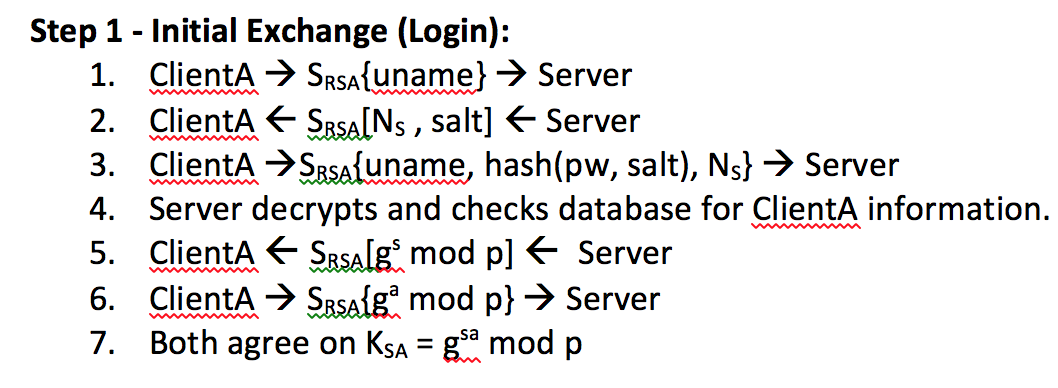
\includegraphics[scale=0.5]{login}
\end{flushleft}
 
\bigskip
 
\subsection{RETREIVING BUDDY LISTS}
\begin{flushleft}
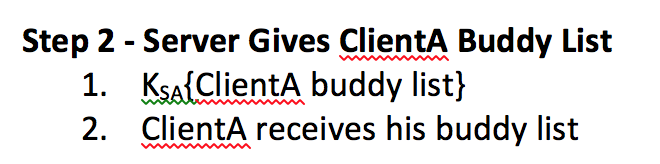
\includegraphics[scale=0.5]{buddies}
\end{flushleft}
 
 \bigskip
 
\subsection{CLIENT-CLIENT SESSION ESTABLISHMENT}
\begin{flushleft}
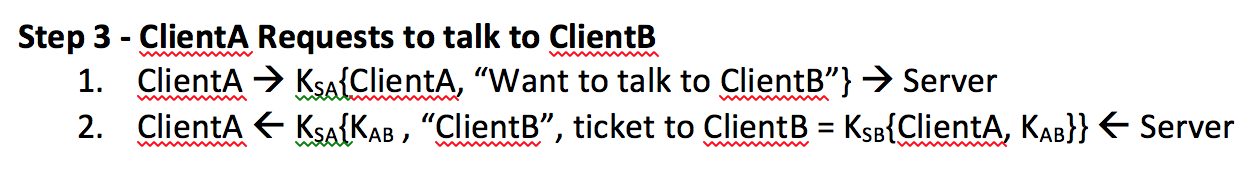
\includegraphics[scale=0.5]{clientreq}
\end{flushleft}
 
\bigskip
 
\subsection{MUTUAL AUTHENTICATION}
During mutual authentication, order of the clients in the encrypted message with the shared session key between
the clients matters. The first client in the message is the originating client while the second client in the message
is the destination client. That means, switching the order can allow authentication of the clients.
\begin{flushleft}
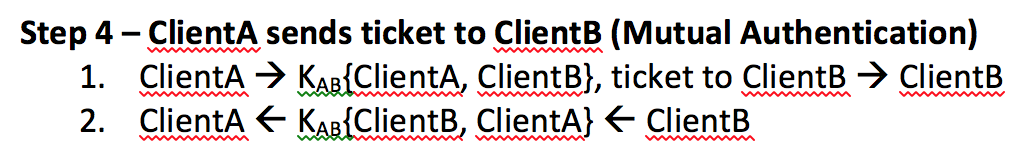
\includegraphics[scale=0.5]{mauth}
\end{flushleft}
 
\bigskip
 
\subsection{DERIVING ENCRYPTION/AUTHENTICATION KEYS}
\begin{flushleft}
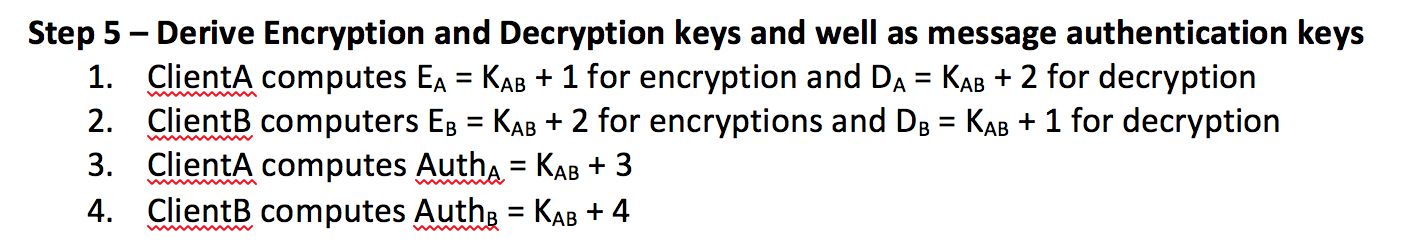
\includegraphics[scale=0.5]{keys}
\end{flushleft}
\end{document}
